\documentclass[screen,nonacm]{acmart}

\usepackage{booktabs}
\usepackage{hyperref}
\usepackage{lipsum}
\usepackage{multicol}
\usepackage{tcolorbox}
\usepackage{xcolor}
\usepackage{adjustbox}
\usepackage{tikz}
\usetikzlibrary{positioning,shapes,arrows}

\usepackage{minted}
\setminted{
    autogobble=true,
    breaklines=true,
    fontsize=\small,
    xleftmargin=2em
}


\begin{document}

\title{
  TAGE Branch Predictor on Sniper Simulator
}
\subtitle{
  CS5222 -- Project 1
}

\author{Shen Jiamin (A0209166A)}
\email{shen_jiamin@u.nus.edu}


% \begin{abstract}

%   Implementing the branch predictor in Sniper will allow us to learn the details of a novel
%   branch predictor. What I feel is important for this project is the quality of the comparison
%   against existing branch predictors, as well as whether the benchmarks meet the expected
%   performance from the reviewed paper. In addition, describing the key features of the
%   branch predictor chosen is an important part of this project. Why did you choose this
%   predictor? Below are some examples of some questions that I’d like to see answers to in
%   your report (adding more background / description / results are a plus and will help your
%   grade).
%   \begin{itemize}
%     \item[\checkmark]
%       Why did you choose this branch predictor?
%     \item[\checkmark]
%       What are interesting components of this branch predictor?
%     \item[\checkmark]
%       What was novel about this predictor when it was published?
%       While a critical review is not necessary for this report, an in-depth overview is
%       needed.
%     \item[\checkmark] What branch predictors were this one compared to in the original paper?
%     \item Did your implementation perform as expected?
%     \item[\checkmark] How did you debug your implementation?
%     \item[\checkmark] Please compare this branch predictor against the two other branch predictors in
%           Sniper, and plot as an MPKI miss chart (misses per 1K instructions) for each of the 5
%           benchmarks and 3 branch predictors.
%     \item Bonus, implement the branch predictor that was compared to in the paper (the one
%           that was beaten) so that we can compare performance numbers against the original
%           (20\% bonus).
%   \end{itemize}

% \end{abstract}

\maketitle

\section{Introduction}

In the paper ``A case for (partially) TAgged GEometric history length branch
prediction'' \cite{Seznec06jilp} by Andr{\'e} Seznec (2006),
the author presented his design of a new branch predictor named TAGE predictor.
% Background
The paper was produced in the background that
(1) exploiting several different history lengths is acknowledged, and
(2) hybrid predictors combining the prediction result from multiple meta predictors have been developed as well as prediction combination functions such as majority vote, predictor fusion and partial tagging and the adder tree seems to outstanding among them.

% Contribution
The TAGE predictor users a geometric series as the list of history length,
which is the main characteristic of O-GEHL\cite{Seznec05isca},
while it derives the main structure from PPM-like predictor\cite{Michaud05jilp}.
%
The significant difference of TAGE from O-GEHL is the use of partial tags instead of adder tree, which the author believes provides better accuracy and storage efficiency and enables the adaptation of the design for conditional branch prediction to the indirection target branch prediction.
Compared with the PPM-like predictor, TAGE proposed a new predictor update algorithm that minimizes the perturbation induced by a single occurrence of a branch.
%
Based on the structure of TAGE, the author also proposed an indirect branch target predictor ITTAGE and a unified predictor COTTAGE, which supports both conditional branch and indirect branch target prediction.

% Evaluation
The author evaluated the accuracy of the TAGE predictor with the parameters listed in Table 2 in the paper.
He compared the MPKI (mispredictions per kilo instructions) of TAGE, O-GEHL\cite{Seznec05isca} and PPM-like\cite{Michaud05jilp} predictors with different prediction tables sizes.
The result shows that the TAGE predictor outperforms O-GEHL and PPM-like in all tested conditions, indicating the correctness of the author's proposal.
He also evaluated the accuracy regarding the variation of history length, which shows that with the maximum history length growing, the accuracy is better at first but no improvement when the length is too long.
The evaluation plot for the impact of the tag width is not as clear as the ones ahead.
The variation of interest is the tag width, but the plot's x-axis varies the prediction tables size, which makes it difficult to compare between different tag widths.
The result shows that increasing the tag width over a threshold provides little return for accuracy improvement.
Besides the explicit evaluations discussed above, the experiment results show that the mispredictions decrease with larger prediction tables but diminishing returns for accuracy.

% Assumption

% Conclusion
The work is auspicious in that many variations of TAGE predictor are proposed after it and lead nearly all the Championship Branch Prediction afterwards, for example, L-TAGE\cite{Seznec07jilp} in 2007, ISL-TAGE\cite{Seznec11hal} in 2011 and TAGE-SC-L\cite{Seznec14hal,Seznec16hal} in 2014 and 2016.

% Limitation
However, these following works also indicate the limitations of the TAGE predictor.
In \cite{Seznec07jilp}, the author found that using the alternate prediction, instead of the prediction using the longest history, for newly allocated entries is more efficient in some applications.
He also identified that TAGE fails to predict when the control flow path inside the loop body is irregular and augmented TAGE with loop predictor.
In \cite{Seznec11hal}, it is identified that TAGE sometimes fails to predict branches that are not strongly biased but that are only statistically biased and thus the Statistical Corrector Predictor is introduced.
He also identified that the number of access to the predictor can be reduced and had an Immediate Update Mimicker as an add-on.

I choose this branch predictor because it's the base of many TAGE-variant branch predictors.
Having this implemented in Sniper will make the following implementations for the variants easier.
The most difficult part in implementing TAGE is the design of the hash functions used to generate the indices and tags,
which is completely not described in the paper.

\section{TAGE Branch Predictor}

\subsection{Structure}

A \(N\)-component TAGE branch predictor consists of one base predictor and \(N-1\) tagged predictor components.

The base predictor is a simple bimodal branch predictor.
A bimodal branch predictor is an array of saturating signed counters.
The counters are indexed only by the program counter.

A tagged predictor component is an array of \textsf{(ctr, tag, u)} 3-tuples.
\textsf{ctr} is a prediction counter like the ones in the bimodal predictor.
It is a saturating signed counter indicating the branch tendency.
\textsf{u} is a usefulness counter.
It is a saturating unsigned counter indicating how useful the entry is.
A tagged predictor component uses two difference hash functions to index the table
and generate tags.
Both of the two hash functions take the program counter and the prediction history as its inputs.
Importantly, the tagged components keeps prediction histories of different lengths,
where the lengths are a geometric series.



\subsection{Prediction Algorithm}

The prediction is produced by combining the prediction result from all the components.

The base predictor, which doesn't make prediction based on prediction history,
produce the prediction result by directly checking if the indexed counter is non-negative.
If $\mathsf{ctr} \ge 0$, the predictor returns a \texttt{taken} prediction.

The tagged components, which make prediction based on prediction histories of different lengths,
produce the prediction result by first checking if the indexed entry has a matched tag with regards to the current program counter and prediction history,
and returns no prediction if the tag doesn't matched.
With a matched tag, it returns a \texttt{taken} prediction if $\mathsf{ctr} \ge 0$.

Among the predictions from the components,
TAGE takes the one based on the longest prediction result as the prediction result.
That is, the last component that provides a prediction.
The component that provides the final prediction is the \textbf{provider component},
and the component that would have provided the prediction, if the provider component does not, is the \textbf{alternative component}.


It should be noted that TAGE can always give a prediction because it will fallback
to bimodal predictor if all the tagged components fail to match the tag,
while a bimodal predictor can always provide a prediction.

\subsection{Update Algorithm}


Assume that the prediction provided by provider component is \textsf{hitpred}
and the one provided by alternative component is \textsf{altpred}.
The actual branch result is \textsf{actual}.

\subsubsection{Update Base Predictor}

The bimodal predictor is always updated by incrementing its \textsf{ctr} if the branch result
is \textsf{taken} or decrementing the \textsf{ctr} if the branch result
is \textsf{not taken}.

\subsubsection{Update Usefulness Counter}
The usefulness counter is updated on two cases.
\begin{enumerate}
  \item If $\mathsf{hitpred} \ne \mathsf{altpred}$ and the provider component is a tagged component,
        the indexed entry from the provider component should update its usefulness counter.
        The counter is incremented if the prediction is correct ($ \mathsf{hitpred} = \mathsf{actual} $),
        which means it's more useful, and decremented otherwise.
  \item Periodically, the usefulness counter should be reset to imitate the
        behavior of Least Recently Used policy.
        Concretly, every call to update function will increment a \texttt{tick} counter.
        When it hits a threshold, it clears the least significant bit (or most significant bit, in turn) of all the usefulness counters in all components.
\end{enumerate}

\subsubsection{Update Prediction Counter}

If the provider component is a tagged component,
the indexed entry in the provider component will update its \textsf{ctr}.
It increments \textsf{ctr} if the branch result is \textsf{taken}
and decrementing the \textsf{ctr} otherwise.

\subsubsection{Allocate New Entry}

The predictor attempts to allocate a new entry
if the prediction is incorrect ($ \mathsf{hitpred} \ne \mathsf{actual} $)
and the provider component didn't keep the longest prediction history.
When allocating a new entry, the predictor looks for an available component,
where the entry indexed has a usefulness count of 0,
from the components taking longer history than the provider component.

If there are multiple components available, the predictor chooses one randomly.
The components taking longer history has a higher probability of being chosen.
If there is no available components,
all the usefulness counter in these components are decremented.

\section{Debugging}

As the build system for sniper is confusing for me, I chose to use ``Caveman Debugging''.
This is done by printing the critical states during execution and examine their behavior.
One successful example is when I printed out the distribution of hit component,
I found that the prediction is heavily based on the bimodal predictor,
while only less than 1/1000 go to the tagged components.
This is very strange and inspired me to examine the allocating behavior and the calculation of indices and tags.
It turns out that I incorrectly implemented the global prediction history buffer,
which caused a significant loss of history information.

\section{Evaluation}

\subsection{Parameter Search}

The first part of the evaluation aims to search for a configuration that makes TAGE works well.
The two selected number of tagged components are 5 and 8, and the bit lengths of \textsf{tag} are 9 and 11 respectively.
The bit length of \textsf{ctr} is set to 4,
With \(n \in [15,24) \), we set the log length of bimodal prediction table as \( n-4 \) while
the log length of tagged prediction table as \(n-6\).
and the minimun length of history is set to 4.
The space for maximum length of history is \(
\left\{  32, 64, 128, 256, 512, 1024, 2048  \}\right\}
\).
The results are plot in \autoref{fig:tage5} and \autoref{fig:tage8},
whico show that the TAGE predictor works best with the configuration listed in \autoref{table:config-1b}.


\begin{figure}
  \centering
  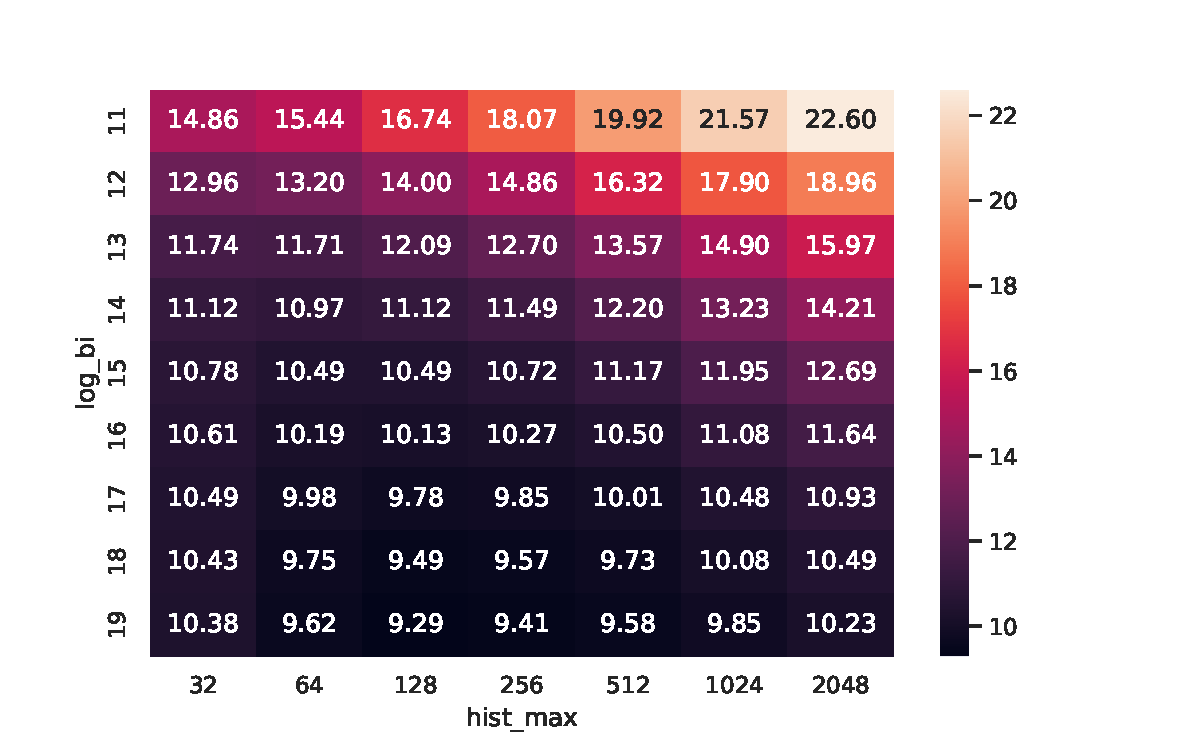
\includegraphics[width=0.64\linewidth]{images/tage5.pdf}
  \caption{Result of parameter search with 5 tagged components (The annotated number is MPKI)}\label{fig:tage5}
\end{figure}

\begin{figure}
  \centering
  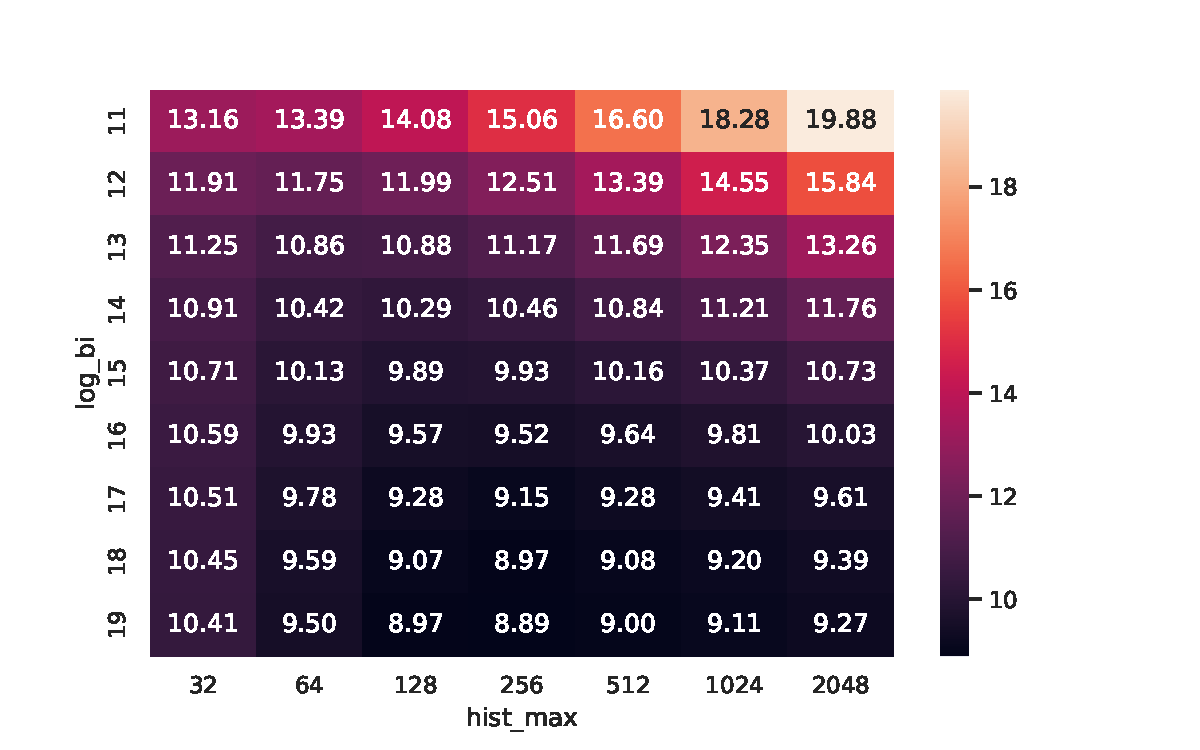
\includegraphics[width=0.64\linewidth]{images/tage8.pdf}
  \caption{Result of parameter search with 8 tagged components (The annotated number is MPKI)}\label{fig:tage8}
\end{figure}


The plot also shows that if the maximum history length is too long,
which leads to inclusion of unrelated prediction history during prediction,
the prediction performance may goes worse.


\subsection{Comparision}


\begin{table}
  \caption{Configuration of TAGE predictors in comparison}
  \label{table:config-1b}
  \centering
  \begin{tabular}{l|cc}
    \toprule
    Parameter                                     & TAGE-5   & TAGE-8   \\
    \midrule
    \# Tagged Components                          & 5        & 8        \\
    \# of entries in Bimodal Predictor (\(\log\)) & 19       & 19       \\
    \textsf{ctr} + \textsf{tag} width (bits)      & 3 + 9    & 3 + 11   \\
    \# of entries in Tagged Components (\(\log\)) & 17       & 17       \\
    History length (bits)                         & 4 -- 128 & 4 -- 256 \\
    Misprediction Penalty                         & 8        & 8        \\
    \bottomrule
  \end{tabular}
\end{table}


We also have a comparison between the implemented TAGE branch predictor and other predictors existing in the Sniper.
We configured two different of TAGE predictors, named TAGE-5 and TAGE-8 as shown in \autoref{table:config-1b}.
Then we run 1B instructions based on ``nehalem-lite'' configuration of Sniper and simulate the five provided pinballs.
The simulation result is shown as \autoref{fig:1b}.

Due to some unknown causes, the pinballs exit earlier without completing the 1B-instruction simulation.
Among the five pinballs, only bzip2 and mcf can complete the simulation for \(1 \times 10^9 \) instructions.
The number of instructions simluated for the pinballs is attached in the parentheses.

By comparing the MPKI (misses per 1K instructions), we find that TAGE-5 and TAGE-8 have similar performance.
They outstand in gobmk and sjeng simulation and worse only than Pentium M in other simulations.

\begin{figure}
  \centering
  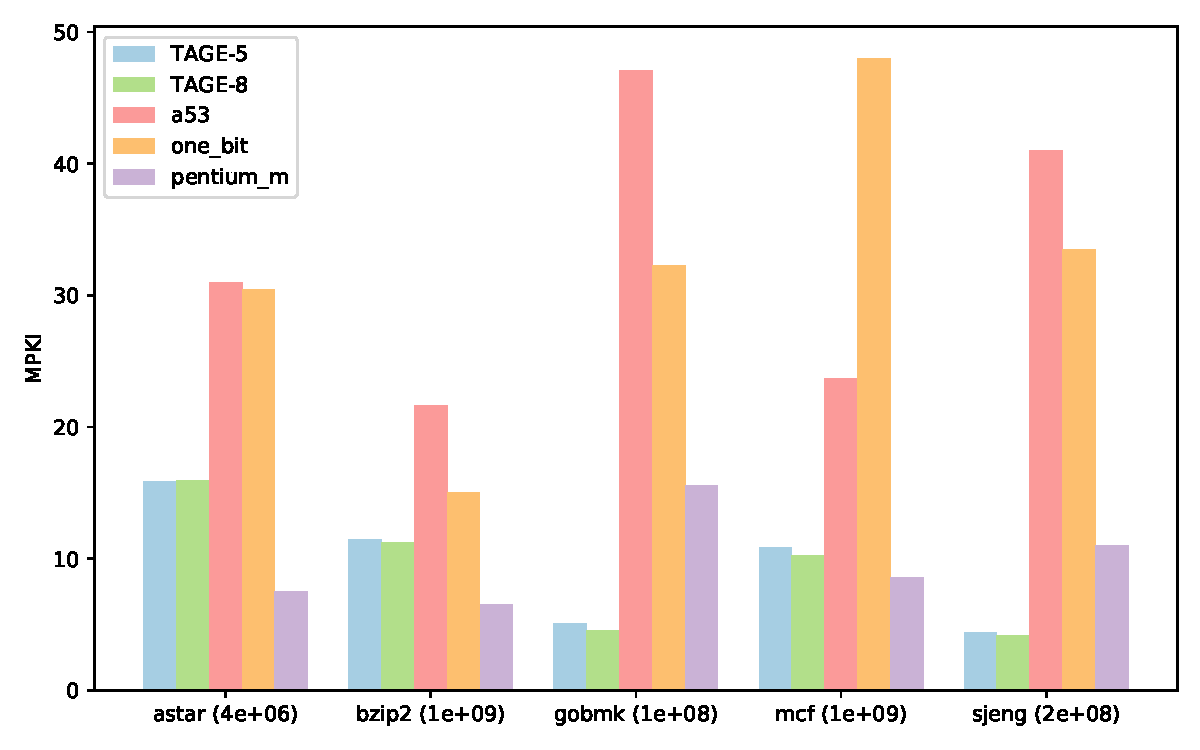
\includegraphics[width=0.64\linewidth]{images/1B.pdf}
  \caption{Comparision of different predictors on the pinballs}\label{fig:1b}
\end{figure}


\begin{acks}
  I'm willing to get my work merged into the Sniper codebase.
\end{acks}

\bibliographystyle{ACM-Reference-Format}
\bibliography{base}

\newpage

\appendix

\end{document}
\endinput
